\documentclass[aspectratio=169,12pt]{beamer}
\usetheme{Madrid}
\usecolortheme{dolphin}
\usefonttheme{professionalfonts}
\setbeamertemplate{navigation symbols}{}
\setbeamertemplate{footline}{}

\usepackage[T1]{fontenc}
\usepackage[utf8]{inputenc}
\usepackage{graphicx}
\usepackage{amsmath,amssymb}
\usepackage{hyperref}
\usepackage{siunitx}
\usepackage{physics}
\usepackage{braket}

\graphicspath{{../../figures/}}

\title[Module A3]{Module A3: La mesure}
\author{JAMOTTE Maxime, SCHOONEN Cédric}
\institute{Digital Learning Hub}
\date{}

\begin{document}

\begin{frame}
  \titlepage
\end{frame}

\begin{frame}{Objectifs du module A3}
    \begin{itemize}
        \item La mesure comme projection (dans la base computationnelle)\\~\\
        \item Visualisation géométrique\\~\\
        \item Notation algébrique: produit scalaire, bra, et projecteurs\\~\\
        \item Reproductibilité de la mesure\\~\\
        \item Projection sur des vecteurs arbitraires: autres bases et observables
    \end{itemize}
\end{frame}

% ============================================================
\section{La mesure comme projection}
% ============================================================

\begin{frame}{Mesurer un qubit}
  \begin{itemize}[<+->]
    \setlength{\itemsep}{0.6em}
    \item État général d'un qubit: $\ket{\psi} = \alpha \ket 0 + \beta \ket 1$.
    \\~\\
    \item Mesurer un qubit donne \textbf{un seul résultat}: $\ket{0}$ ou $\ket{1}$ (dans la base computationnelle).
    \\~\\
    \item Les probabilités sont données par le \textbf{carré des coefficients}:
    $$P(\ket 0) = |\alpha|^2, \qquad P(\ket 1) = |\beta|^2$$
    \item Après la mesure, l'état est \textbf{projeté} sur le résultat obtenu ($\ket{0}$ ou $\ket{1}$).
  \end{itemize}
\end{frame}

% ============================================================
\section{Visualisation géométrique}
% ============================================================

\begin{frame}{Produit scalaire}
  \begin{columns}[T]
    \begin{column}{0.6\textwidth}
      \begin{itemize}
        \setlength{\itemsep}{0.6em}
        \item La probabilité d'obtenir un résultat de mesure vient (en gros) d'une comparaison de deux états quantiques.
        \item Cette comparaison se traduit par un produit scalaire entre leurs vecteurs associés.
        $$\vec r \cdot \vec p = \begin{pmatrix} a & b \end{pmatrix} \begin{pmatrix} c \\ d \end{pmatrix} = ac+bd$$
        \item Lien avec l'angle: $\vec r \cdot \vec p = \norm{\vec r}\norm{\vec p}\cos(\theta)$.
        \item Produit scalaire entre deux états $\ket{\phi}$ et $\ket \psi$: $\braket{\phi|\psi}$.
        \item Conventions: $\braket{0|0} = 1$, $\braket{1|1} = 1$ et $\braket{0|1} = 0$ (orthogonaux).
      \end{itemize}
    \end{column}
    \begin{column}{0.35\textwidth}
      \centering
      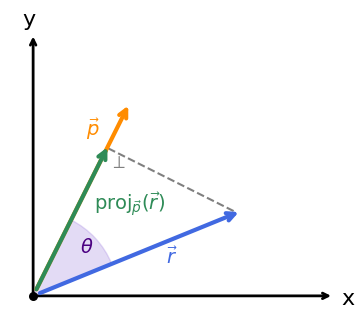
\includegraphics[width=\linewidth]{proj.png}
    \end{column}
  \end{columns}
\end{frame}

% ============================================================
\section{Notation algébrique: projecteurs}
% ============================================================

\begin{frame}{Mesurer en mécanique quantique}
  \begin{itemize}[<+->]
    \item Si $\ket \psi = a \ket 0 + b \ket 1$ et $\ket \phi = c \ket 0 + d \ket 1$ alors:
    \begin{equation*}
      \begin{split}
        \braket{\phi|\psi}
        &= \begin{pmatrix}
          a\  b
        \end{pmatrix}
        \begin{pmatrix}
          c\\d
        \end{pmatrix} = ac \braket{0|0} + ad \braket{1|0} + bc \braket{0|1} + bd \braket{1|1} = ac +bd\\
        &= \vec r_\phi^{} \cdot \vec p_\psi^{} = \|\vec r_\phi^{}\|\ \|\vec p_\psi^{}\| \cos(\theta)
      \end{split}
    \end{equation*}
    \item \textbf{Postulat}: mesurer = projeter le vecteur du qubit sur le vecteur propre associé à la
     valeur propre de l'observable mesurée.\\~\\
    \item On projette avec un projecteur $\Pi_{\phi}^{} = \ket \phi \bra \phi$ sur l'état $\phi$: $\ket \phi \braket{\phi|\psi}$.\\~\\
    \item Probabilité de mesurer la valeur propre = le produit scalaire entre état projeté et état initial: 
    $$ \bra \psi \Pi_\phi \ket \psi = \braket{\psi|\phi}\braket{\phi|\psi} = |\braket{\phi|\psi}|^2 $$
  \end{itemize}  
\end{frame}

\begin{frame}{Projecteurs en notation matricielle}
  \begin{itemize}[<+->]
    \setlength{\itemsep}{0.6em}
    \item Les projecteurs $\Pi_0$ et $\Pi_1$ s'écrivent aussi comme des matrices $2\times 2$:
    $$\Pi_0 = \ket{0}\bra{0} =
      \begin{pmatrix}1\\0\end{pmatrix}\begin{pmatrix}1 & 0\end{pmatrix}
      = \begin{pmatrix}1 & 0\\0 & 0\end{pmatrix}$$
    $$\Pi_1 = \ket{1}\bra{1} =
      \begin{pmatrix}0\\1\end{pmatrix}\begin{pmatrix}0 & 1\end{pmatrix}
      = \begin{pmatrix}0 & 0\\0 & 1\end{pmatrix}$$
    \item On vérifie la relation de complétude:
    $\Pi_0 + \Pi_1 = \begin{pmatrix}1 & 0\\0 & 1\end{pmatrix} = I$ (matrice identité).
    \item La probabilité de mesurer $\ket{0}$ s'écrit:
    $P(0) = \bra{\psi}\Pi_0\ket{\psi} = |\alpha|^2$.
  \end{itemize}
\end{frame}

% ============================================================
\section{Reproductibilité de la mesure}
% ============================================================

\begin{frame}{Reproductibilité de la mesure: $\Pi^2 = \Pi$}
  \begin{itemize}[<+->]
    \setlength{\itemsep}{0.8em}
    \item La mesure \textbf{projette} l'état quantique sur $\ket{0}$ ou $\ket{1}$
     selon les probabilités $P(\ket 0)$ et $P(\ket 1)$. \textbf{Le système est définitivement dans un des états propres}.\\~\\
    \item Si on mesure à nouveau, on retrouve le même résultat: la mesure est reproductible.\\~\\
    \item Mathématiquement: $\Pi^2 = \Pi$ (idempotence du projecteur), c'est pourquoi la mesure est une projection.
  \end{itemize}
\end{frame}

\begin{frame}{Valeurs propres et vecteurs propres}
  \begin{itemize}[<+->]
    \setlength{\itemsep}{0.6em}
    \item Cas particuliers d'un produit matrice-vecteur:   
    $$ \begin{pmatrix} 2 & 1 \\ 2 & 3 \end{pmatrix} \begin{pmatrix} -1 \\ 1 \end{pmatrix} = \begin{pmatrix} -1 \\ 1 \end{pmatrix},$$
    et 
    $$ \begin{pmatrix} 2 & 1 \\ 2 & 3 \end{pmatrix} \begin{pmatrix} 1 \\ 2 \end{pmatrix} = \begin{pmatrix} 4 \\ 8 \end{pmatrix} = 4 \begin{pmatrix} 1 \\ 2 \end{pmatrix},$$~\\
    \item Multiplier ce vecteur par cette matrice redonne le même vecteur multiplié par un nombre.
    \item On nomme ce vecteur "\textbf{vecteur propre}" et ce nombre "\textbf{valeur propre}".
  \end{itemize}
\end{frame}

\begin{frame}{Les états sont des vecteurs propres d'une observable}
  \begin{itemize}[<+->]
    \setlength{\itemsep}{0.6em}
    \item Les grandeurs mesurables sont représentées par des matrices appelées \textit{observables}.
    \item \textbf{Mesurer} une quantité physique revient à mesurer l'une de ses \textbf{valeurs propres}.
    \item Les états $\ket{0}$ et $\ket{1}$ sont les vecteurs propres de l'observable $Z$
     (base computationnelle):
    $$Z\ket{0} = +\ket{0}, \qquad Z\ket{1} = -\ket{1}$$
    \item La nature physique de la valeur propre (énergie, spin,...) dépend de la plateforme (voir module D1).
  \end{itemize}
\end{frame}

% ============================================================
\section{Autres bases et observables}
% ============================================================

\begin{frame}{Projection sur des vecteurs arbitraires}
  \begin{itemize}[<+->]
    \setlength{\itemsep}{0.8em}
    \item On peut mesurer dans d'autres bases que la base computationnelle $\{\ket{0}, \ket{1}\}$.\\~\\
    \item Par exemple, la base $\{\ket{+}, \ket{-}\}$ avec:
    $$\ket{+} = \frac{\ket{0}+\ket{1}}{\sqrt{2}}, \qquad \ket{-} = \frac{\ket{0}-\ket{1}}{\sqrt{2}}$$
    \item Les vecteurs $\ket{+}$ et $\ket{-}$ sont les vecteurs propres de l'observable $X$:
    $$X\ket{+} = +\ket{+}, \qquad X\ket{-} = -\ket{-}$$
    \item On peut ainsi définir des projecteurs et probabilités de mesure dans cette base.
  \end{itemize}
\end{frame}

\begin{frame}{Fin du module A3}
    \begin{itemize}
        \item La mesure comme projection (dans la base computationnelle)\\~\\
        \item Visualisation géométrique\\~\\
        \item Notation algébrique: produit scalaire, bra, et projecteurs\\~\\
        \item Reproductibilité de la mesure\\~\\
        \item Projection sur des vecteurs arbitraires: autres bases et observables
    \end{itemize}
\end{frame}

\end{document}
